%%%%%%%%%%%%%%%%%%%%%%%%%%%%%%%%%%%%%%%%%%%%%%%%%%%%%%%%%%%%%%%%%%%%%%%%%%%%%%
\documentclass[12pt,hidelinks]{article}

% 1. Load LaTeX packages
\usepackage{fontspec}
\usepackage{geometry}
\usepackage{lastpage}
\usepackage{fancyhdr}
\usepackage{hyperref}
\usepackage{amsmath}
\usepackage{amsthm}
\usepackage{xunicode}
\usepackage{listings}
\usepackage{color}
\usepackage{amssymb}

% 2. Define page dimensions and spacing
\geometry{top=1in, bottom=1in, left=1in, right=2in, marginparsep=4pt,
          marginparwidth=1in}
\setlength{\parindent}{0pt}
\setlength{\parskip}{12pt}

% 3. Set header, footer, and bibliography
\renewcommand{\headrulewidth}{0pt}
\pagestyle{fancyplain}
\fancyhf{}
\lfoot{}
\rfoot{page \thepage\ of \pageref{LastPage}}
\bibliographystyle{acm}

% 4. Set fonts for the document
\defaultfontfeatures{Mapping=tex-text}
\setromanfont{YaleNew}

% 5. Define custom code for book environments and commands
\DeclareMathOperator*{\argmin}{arg\,min}
\DeclareMathOperator*{\argmax}{arg\,max}
\newcommand{\code}[1]{\texttt{#1}}
\newcommand{\pkg}[1]{\textbf{#1}}

% 6. Define custom code for book environments and commands
\definecolor{verbgray}{gray}{0.9}
\definecolor{verbgray2}{gray}{0.975}

\lstnewenvironment{rcode}{%
  \lstset{backgroundcolor=\color{verbgray},
  frame=single,
  framerule=0pt,
  basicstyle=\ttfamily,
  keepspaces=true,
  columns=fullflexible}}{}

\lstnewenvironment{rres}{%
  \lstset{backgroundcolor=\color{verbgray2},
  frame=single,
  framerule=0pt,
  basicstyle=\ttfamily,
  keepspaces=true,
  columns=fullflexible}}{}

% 7. Define numbering scheme for equations (only needed for handout).
\numberwithin{equation}{section}
\setcounter{section}{1}

%%%%%%%%%%%%%%%%%%%%%%%%%%%%%%%%%%%%%%%%%%%%%%%%%%%%%%%%%%%%%%%%%%%%%%%%%%%%%%
\begin{document}

{\LARGE Handout 02: Linear Regression (Optional)}

\vspace*{18pt}


\textbf{Vectors}

For us, a vector is simple an ordered collection of real numbers. The number
of terms in the collection is called the \textit{dimension} of the vector and
we write $v \in \mathbb{R}^n$ to represent an $n$-dimensional vector $v$. You
can think of the vector as a column of number:
\begin{align}
v &= \begin{bmatrix} v_1 \\ v_2 \\ \vdots \\ v_n \end{bmatrix} \in \mathbb{R}^n.
\end{align}
We use the notation $v_i$ to refer to the $i$'th term in the vector. Vector
addition is defined \textit{componentwise} such that:
\begin{align}
v + u &= \begin{bmatrix} v_1 \\ v_2 \\ \vdots \\ v_n \end{bmatrix} +
\begin{bmatrix} u_1 \\ u_2 \\ \vdots \\ u_n \end{bmatrix}
=\begin{bmatrix} v_1 + u_1 \\ v_2 + u_2 \\ \vdots \\ v_n + u_n \end{bmatrix}
\end{align}
Only vectors of the same dimension can be added together. We can also multiply
a vector by a fixed scalar value $\alpha \in \mathbb{R}$ in a component-wise
fashion:
\begin{align}
\alpha \cdot v &= \alpha \cdot \begin{bmatrix} v_1 \\ v_2 \\ \vdots \\ v_n \end{bmatrix}
= \begin{bmatrix} \alpha \cdot v_1 \\ \alpha \cdot v_2 \\ \vdots \\ \alpha \cdot v_n \end{bmatrix}.
\end{align}
It is possible to define a component-wise multiplication of two vectors, but
this is rarely very useful and we will skip this for now.

We can also describe the size of a vector by thinking of the distance between
the set of numbers in $n$-dimensional space and the origin. Specifically, the
Euclidean-norm (or $\ell_2$-norm) of a vector is given and defined by:
\begin{align}
|| v ||_2 &= \sqrt{\sum_i v_i^2}.
\end{align}
This should correspond with other definitions you may have seen for distance
measures. Finally, we will also define the inner product between two vectors
of the same dimension as:
\begin{align}
u \cdot v &= \sum_i u_i v_i.
\end{align}
This form will be most useful for us, but its helpful to also visualize the
dot product geometrically by its equivalent form:
\begin{align}
u \cdot v &= || u ||_2 \cdot || v ||_2 \cdot cos(\theta)
\end{align}
For the angle $\theta$ between the two vectors; of particular note, the dot
product is zero for perpendicular vectors. Note that the Euclidean-norm can
be defined by using the dot product of a vector with itself:
\begin{align}
v \cdot v &= \sum_i v_i v_i = || v ||_2^2
\end{align}
There is a lot of other very interesting and useful geometric intuition behind
these definitions that we don't have time to get into right now. Hopefully
some of these will arise as we work through the next few weeks and you will
see how they apply to linear regression theory.

\textbf{Gradient}

Assume that we have a real valued function $f$ defined on $n$-dimensional
vectors. In other words:
\begin{align}
f: \mathbb{R}^n \rightarrow \mathbb{R}.
\end{align}
The gradient of $f$, denoted by $\nabla f$, is given by the vector of partial
derivatives with respect to each component:
\begin{align}
\nabla f &= \begin{bmatrix} \frac{\partial f}{\partial v_1} \\
 \frac{\partial f}{\partial v_2}  \\ \vdots \\
 \frac{\partial f}{\partial v_n}  \end{bmatrix}
\end{align}
As with first derivatives, we can use the gradient to find the critical point
of a multivalued function. Understanding gradient is very important for
statistical learning. A typical workflow consists of computing the
gradient of the loss function, $\nabla \mathcal{L}$, trying to set this to
zero, and then evaluating the output.

\textbf{Matrices}

Consider a function that takes as an input vectors of dimension $n$ and returns
as an output vectors of dimension $m$:
\begin{align}
M: \mathbb{R}^m \rightarrow \mathbb{R}^n.
\end{align}
We say that $M$ is a linear function if we can take scalar quantities outside
of the function,
\begin{align}
M(\alpha \cdot x) &= \alpha \cdot M(x), \quad x\in \mathbb{R}^m, \alpha \in \mathbb{R},
\end{align}
And we can split vector sums across the function,
\begin{align}
M(x + y) &= M(x) + M(y), \quad x, y\in \mathbb{R}^n.
\end{align}
It turns out that any such map can be described a grid of numbers with $n$ rows
and $m$ columns:
\begin{align}
M &= \begin{bmatrix} m_{1,1} & m_{1,2} & \cdots & m_{1,m} \\
m_{2,1} & \ddots & \cdots & m_{2,m} \\
\vdots  & \vdots & \ddots & \vdots \\
m_{n, 1} & m_{n, 2} & \cdots & m_{n, m}
\end{bmatrix}
\end{align}
By defining:
\begin{align}
M(v)_j &= \sum_i m_{i,j} \cdot v_i \in \mathbb{R}.
\end{align}
You can think of this as taking the dot product of the $j$'th row of the matrix
$M$ and the input vector $v$. Notice that we are abusing notation by letting
$M$ be the grid of numbers \textit{and} the function. This is intentional
because we will use the notation:
\begin{align}
M(v) = Mv \in \mathbb{R}^n, \quad v\in\mathbb{R}^m.
\end{align}
To represent the action of applying the function described by a matrix $M$ to
a vector $v$.

As with vectors, we could spend a whole year just talking about matrices.
Rather than an exhaustive treatment, I want to instead quickly describe a
few properties and notations that we will most useful. First, matrix multiplication
is defined by function composition. The matrix product $A \cdot B$ is defined
as the matrix that corresponds to applying the linear function defined by
$B$ and then applying the linear function implied by $A$. Note that this can
only be defined with the number of columns in $A$ matches the number of rows
in $B$ (why?). If we set $C = A \cdot B$, then the following formula corresponds
to this functional interpretation:
\begin{align}
c_{i, j} &= \sum_k a_{i, k} \cdot b_{k, j}
\end{align}
Where lower case letters refer to the elements in the corresponding uppercase
matrices. The matrix product distributes,
\begin{align}
A (B + C) &= AB + AC,
\end{align}
But in general does not commute,
\begin{align}
AB \neq BA.
\end{align}
The identity matrix $I_n$ is given by ones on the diagonal and zeros elsewhere.
For example
\begin{align}
I_3 &= \begin{bmatrix} 1 & 0 & 0 \\ 0 & 1 & 0 \\ 0 & 0 & 1 \end{bmatrix}.
\end{align}
For a square matrix $A$ we have:
\begin{align}
A I_n = I_n A = A.
\end{align}
Finally, the matrix inverse $A^{-1}$ of a square matrix is defined such that
\begin{align}
A^{-1} A = A A^{-1} = I_n,
\end{align}
However the matrix $A^{-1}$ is not guaranteed to exist.

The final notation we need is the matrix transpose, denoted by $A^t$ and
defined simply as flipping the matrix rows and columns. It has the property
that it can be distributed within a summation:
\begin{align}
(A + B)^t &= A^t + B^t.
\end{align}
The transpose of a matrix product can also be distributed but the order of
the matrices is flipped:
\begin{align}
(AB)^t &= B^t A^t.
\end{align}
The transpose is quite useful because we can use it to compute the dot product
in an interesting way.


Linear models are amongst the most well known and often-used methods for
modeling data. They are employed to study the
outcomes of patients in clinical trials, the price of financial
instruments, the lifetimes of fruit flies, and many other
responses from a wide range of fields.
Why are linear models so popular? One important attribute is that
linear models provide a concrete interpretation for all of their
parameters. Take the two variable model for predicting housing sale
prices as a function of total area (in square feet or square meters)
and the number of bedrooms,
\begin{align}
\text{price}_i &= \beta_0 + \beta_1 \cdot \text{area}_i + \beta_2 \cdot \text{bedrooms}_i + \epsilon_i.
\end{align}
The parameters in this model tell us how much the response, price,
changes when one of the predictor variables changes with the other
variable held fixed. Mathematically, we can describe this precisely
using partial derivatives
\begin{align}
\beta_1 &= \frac{\partial \, \text{price}}{\partial \, \text{area}}, \\
\beta_2 &= \frac{\partial \, \text{price}}{\partial \, \text{bedrooms}}.
\end{align}
The model separates the effect of the total size of a house and the
total number of bedrooms. This information is useful to real estate
agents, homeowners, construction companies, and economists.
Linear models also allow for the interpretation of categorical predictors
through the use of indicator variables. If our housing price data also
includes information about whether a given observation is from one of
three neighborhoods, say `uptown,' `downtown,' and `suburbia,' we can
define variables that are one when observation $i$ is in the given
neighborhood and zero otherwise. A linear model with these variables
may be written as
\begin{align}
\text{price}_i &= \beta_0 + \beta_1 \cdot \text{area}_i + \beta_2 \cdot \text{bedrooms}_i + \\ \nonumber
              & \quad  \beta_3 \cdot \text{downtown}_i + \beta_4 \cdot \text{uptown}_i + \epsilon_i.
\end{align}
The parameter $\beta_3$ can still be viewed as a partial derivative, here
representing the difference in the expected price between a house in suburbia
and a house in the downtown neighborhood, if both are the same size and have
the same number of bedrooms.

The relatively simple form of linear models allows for a
great deal of variation in the model assumptions. The $x_i$'s can
be treated as fixed values, a \textit{fixed design}, or they may
be considered to be random variables themselves, as in a
\textit{random design} model. In biological
applications the analysis usually depends on strict independence
between the errors. In time series data, as commonly seen in finance or macroeconomics,
the $\epsilon_i$ are often serially correlated with one another.
Linear models such as the autoregressive integrated
moving average (ARIMA) model and the autoregressive conditional heteroskedasticity
(ARCH) model are used to model time series data with serial correlation
structures. Longitudinal medical studies, where data is collected on
multiple instances from the same cohort of patients over a period of
time, may assume that the errors for observations from the
same subject correlate differently than errors between different
patients. Fixed, random, and mixed effects
models---core statistical methods within certain sub-disciplines in
the sciences and social sciences---are forms of linear models adapted
to handle applications such as resampled data.

Linear models also benefit from a strong theoretical background. The
standard estimators, which we will explore,
can be described in terms of weighted sums of the original data. Under
weak assumptions, we can then draw on the central limit theorem and
large sample theory to construct asymptotically valid confidence
intervals and hypothesis testing frameworks. Importantly, most of this
theory can be extended to the various extensions and complex assumptions
often used in practice. Also, these theoretical tools are useful even
when the primary task is one of prediction. Hypothesis tests aid in
the process of deciding whether to add
or delete a certain variable from a model. Confidence intervals, when
combined with an estimate of the noise variance, are extensible to
prediction intervals. These provide a range of likely values for newly
observed data points, in addition to a singular `best' value. We
will see several ways in which these estimates are useful in practice
when building predictive models.

The standard estimators for
parameters in linear models can be calculated using relatively straightforward
computational approaches. For this reason, linear models
are often used in applications even when many of the aforementioned
benefits do not directly apply. Notice that a linear model must be
linear only relative to the $\beta$ terms. If we have pairs of data
$(x_i, y_i)$ but believe that there is a non-linear relationship
between $x$ and $y$, we could build the model
\begin{align}
y_i &= \beta_0 + \beta_1 \cdot x_i + \beta_2 \cdot x_i^2 + \cdots + \beta_p \cdot x_i^p + \epsilon_i.
\end{align}
Here it is difficult to discern a conceptual interpretation of each
of the $\beta_j$ terms. As a result, it is also hard to make use of
confidence intervals and hypothesis tests concerning them. However,
the linear model framework is incredibly useful as it provides a
computationally tractable way of estimating an arbitrarily complex
relationship, by setting $p$ as large as possible, between our two
variables. Of course, the size of the dataset will limit the ultimate
complexity of the model, but this is true regardless of the particular
approach taken. We will expand at length on this variable expansion
in the coming months.

\textbf{Ordinary least squares}

Many of the advantages of linear models concern the beneficial properties
of the standard estimators used to compute the unknown parameters
$\beta_j$ from observed data. As a next step we would like to explore
the definition of these estimators. To this aim, it will be useful to
provide a compact matrix-based description of a linear model. Throughout
my notes, unless otherwise noted, we use a notation where $n$ is the
sample size, $p$ is the number of variables, $i$ is an index over the
samples, and $j$ is the index over the variables. With this notation a
complete general description of a linear model can be given by
\begin{align}
\widehat{y}_i &= \beta_1 \cdot x_{i,1} + \cdots + \beta_p \cdot x_{i,p}, \quad \forall\,  i = 1, \ldots, n.
\end{align}
Or simply
\begin{align}
\widehat{y}_i &= \sum_j \beta_j \cdot x_{i,j}, \quad \forall\,  i = 1, \ldots, n.
\end{align}
Notice that we do not need to include an explicit intercept term
$\beta_0$. If one is required this can be included by setting
$x_{i,1}$ equal to one for every single observation $i$. Using
matrix notation, we can write the linear model equation
simultaneously for all observations as
\begin{align}
\left(\begin{array}{c}\widehat{y}_1\\ \widehat{y}_2\\ \vdots\\ \widehat{y}_n\end{array}\right) &=
  \left(\begin{array}{cccc}x_{1,1}&x_{2,1}&\cdots&x_{p,1}\\
                           x_{1,2}&\ddots&&x_{p,2}\\
                           \vdots&&\ddots&\vdots\\
                           x_{1,n}&x_{2,n}&\cdots&x_{p,n}\\\end{array}\right)
  \left(\begin{array}{c}\beta_1\\ \beta_2\\ \vdots\\ \beta_p\end{array}\right)
\end{align}
which can be compactly written in terms of a vector $\widehat{y}$ of the responses,
a matrix $X$ of the predictor variables, and a vector $\beta$ of the unknown
parameters
\begin{align}
\widehat{y} &= X \beta.
\end{align}
Beyond compactness, this notation is also useful as many of the computational
properties of linear models can be reduced to linear algebraic properties of
the matrix $X$.

Now, holding to the framework of predictive modelling, we want to know how to
find a good set of values for $\beta$. To do this, we first need to define a loss
function $\mathcal{L}$ that describes how well a prediction is able to predict
values of $y$. Here we use mean squared error:
\begin{align}
\mathcal{L}(\widehat{y}, y) &= \sum_i (y_i - \widehat{y}_i)^2.
\end{align}
Notice that we can re-write this in matrix form following:
\begin{align}
\mathcal{L} &= || y - \widehat{y} ||_2^2.
\end{align}
From which we can input our formula for $\widehat{y}$
\begin{align}
\mathcal{L} &= || y - X \beta ||_2^2. \label{lloss}
\end{align}
It is useful to also define the residual vector $r$, the thing to minimized
in the loss function:
\begin{align}
r &= y - X\beta.
\end{align}
From here, the next steps are:
\begin{enumerate}
\item Expand the definition of the loss function.
\item Take the gradient of $\mathcal{L}$ using the matrix formulae from the last notes.
\item Set the gradient equal to zero and find the optimal value of $\beta$ from
the training data.
\end{enumerate}

\begin{figure}
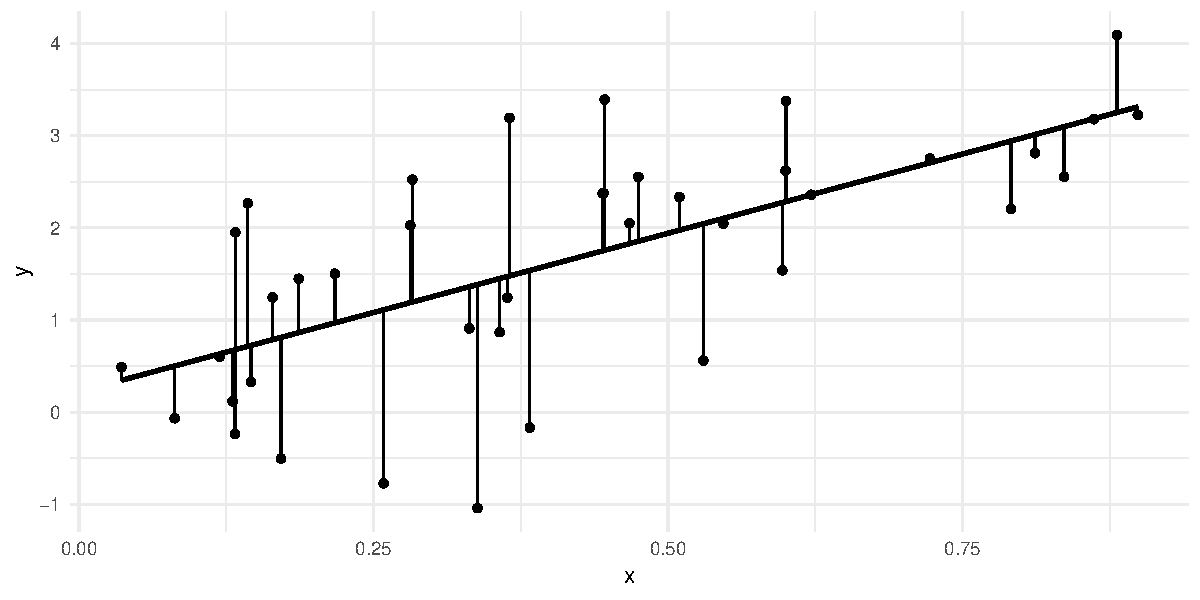
\includegraphics[width=\textwidth]{figures/lm_residuals.pdf}
\caption[Residuals from a simple linear model]{Visualization of residuals
from the linear model $y = \beta_0 + \beta_1 x$.}
\label{lm_residuals}
\end{figure}

\textbf{SVD}

Finally, we are going to work with a particular type of matrix factorization
called the singular value decomposition. Start by assuming that we have a
matrix $A$ with $n$ rows and $p$ columns such that $n \geq p$. The (thin)
singular value decomposition, or SVD, is given by the matrix product:
\begin{align}
A &= U D V^t
\end{align}
With the following dimensions:
\begin{align}
A \in \mathbb{R}^{n \times p} \\
U \in \mathbb{R}^{n \times p} \\
D \in \mathbb{R}^{p \times p} \\
V \in \mathbb{R}^{p \times p}
\end{align}
Furthermore, $D$ is a diagonal matrix with non-negative entries along the
diagonal ordered from the largest to the smallest value:
\begin{align}
D &= \begin{bmatrix}
\sigma_1 & 0 & \cdots & 0\\
0 & \sigma_2 & \cdots & 0 \\
0 & \vdots & \ddots & \vdots \\
0 & 0 & \cdots & \sigma_p \end{bmatrix}, \quad \sigma_1 \geq \sigma_2 \geq \cdots \geq \sigma_p \geq 0.
\end{align}
The values $\sigma_k$ are called the \textit{singular values} of the matrix $A$.
Also, $V$ is an orthogonal matrix such that (we showed in Handout 03 that this
corresponds to a rotation):
\begin{align}
V^t V &= V V^t = I_p.
\end{align}
The matrix $U$ is not square, so it cannot be completely orthogonal, but its
columns are orthogonal to one another so we have:
\begin{align}
U^t U &= I_p.
\end{align}
The singular value decomposition exists for any matrix, and so we can use it
without any assumptions on the matrix we are working with. This has important
geometric implications: \textbf{any} linear function can be written as a
rotation, a fixed scaling of the components, and another rotation.

\textbf{SVD and the Normal Equations}

If we take the SVD of the data matrix $X$, we have
\begin{align}
X &= U D V^t.
\end{align}
Plugging this into the ordinary least squares estimator gives:
\begin{align}
\beta &= (X^t X)^{-1} X^t y \\
&= (V D^t U^t U D V^t)^{-1} V D^t U^t y \\
&= (V D (U^t U) D V^t)^{-1} V D U^t y \\
&= (V D I_p D V^t)^{-1} V D U^t y \\
&= (V D^2 V^t)^{-1} V D U^t y
\end{align}
By taking the fact that a diagonal matrix is its own transpose and using that
$U^t U$ is equal to the identity. Note that $D^2$ is just a matrix with the
squared singular values along the diagonal.

Now, notice that the inverse of $V$ is $V^t$, and vice-versa. Further, the
inverse of $D^{2}$ is equal to a diagonal matrix with the inverse of the
squared singular values along the diagonal (this exists if we assume that
$\sigma_1 > 0$). Therefore:
\begin{align}
(V D^2 V^t)^{-1} &= (V^{t})^{-1} D^{-2} V^{-1} = V D^{-2} V^t
\end{align}
And we can further simplify the equation for the ordinary least squares
estimator:
\begin{align}
\beta &= (V D^2 V^t)^{-1} V D U^t y \\
&= V D^{-2} V^t V D U^t y \\
&= V D^{-2} D U^t y \\
&= V D^{-1} U^t y.
\end{align}
This gives us a compact way to write the ordinary least squares estimator.
It is also far more numerically stable to use this formula to compute the
estimate $\beta$ from a dataset. Most importantly, it will yield a lot of
intuition for what makes some estimation tasks hard and motivate how we can
(partially) address the most challenging regression problems.

\textbf{SVD in R}

In R, you can create the singular value decomposition of a matrix using the
function \texttt{svd}. To see this, let's construct some simulated data:
\begin{rcode}
set.seed(1)
n <- 1e4; p <- 4
X <- matrix(rnorm(n*p), ncol = p)
b <- c(1,2,3,4)
epsilon <- rnorm(n)
y <- X %*% b + epsilon
\end{rcode}
Now, we take the singular value decomposition of the matrix. I will also
explicitly extract out and save the matrices $U$ and $V$ as well as the singular
values $sigma$:
\begin{rcode}
svd_output <- svd(X)
U <- svd_output[["u"]]
V <- svd_output[["v"]]
sigma <- svd_output[["d"]]
\end{rcode}
Now, lets compute the ordinary least square matrix with this data:
\begin{rcode}
beta <- V %*% diag(1 / sigma) %*% t(U) %*% y
beta
\end{rcode}
\begin{rres}
          [,1]
[1,] 0.9870134
[2,] 1.9876739
[3,] 3.0045489
[4,] 4.0102080
\end{rres}
We can verify that this is equivalent to our old form of the estimator by:
\begin{rcode}
solve(t(X) %*% X) %*% t(X) %*% y
\end{rcode}
\begin{rres}
          [,1]
[1,] 0.9870134
[2,] 1.9876739
[3,] 3.0045489
[4,] 4.0102080
\end{rres}
Notice that both are close to the value of \texttt{b} in the simulation.



\end{document}
